\begin{itemize}
    \needspace{10\baselineskip}
	\item \textbf{Simulation Methodology (Dyno Simulation):} \\
	Experimental data was exported into .csv file which was channeled to the chrono model. 
	Real time from the data was synchronized with the simulation timeStep to use the PWM Duty Cycle and the Load Torque as a input.

	All the crucial simulation Parameters used - 
	\begin{align}
	K_t &= 0.005\,\mathrm{Nm/A} \\
	K_v &= 1900\,\mathrm{rpm/V} \\
	\textit{Resistance} &= 0.040\,\Omega \\
	\textit{Inductance} &= 10 \times 10^{-5}\,\mathrm{H} \\
	\textit{PwmFrequency} &= 1\,\mathrm{kHz} \\
	\textit{MechanicalFrequency} &= 10^5\,\mathrm{Hz} \\
	\textit{ElectricalFrequency} &= 10^5\,\mathrm{Hz} \\
	\textit{ElectronicSamplingFrequency} &= 0.005\,\mathrm{Nm/A}
	\end{align}
	
	\begin{figure}[H]
		\centering
		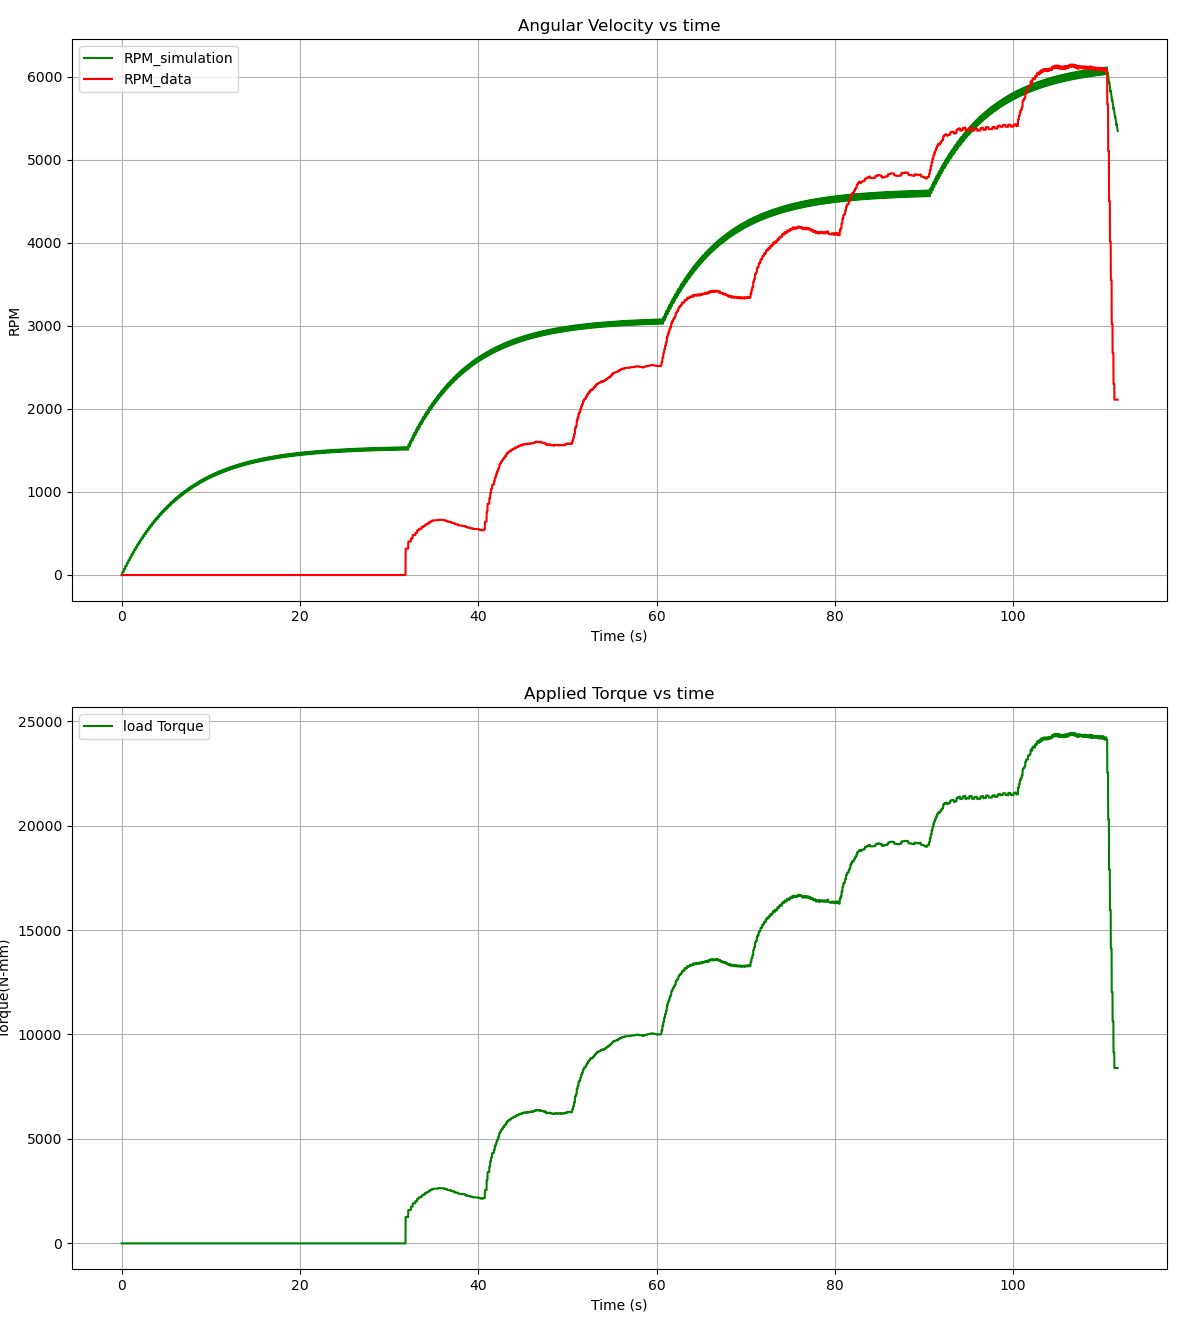
\includegraphics[width=0.75\textwidth]{images/Screenshot From 2025-03-26 07-59-40.png}
	\end{figure}
	\textbf{Observations-} \\
	As we can see the simulation can approximate the Dyno test data almost accurately with some errors. The error can be substantially decreased with further fine tuning of the frequencies, sampling time and the electical motor specifications.
	
    \needspace{10\baselineskip}
	\item \textbf{No load:} 
	
\end{itemize}
\begin{itemize}
	\needspace{10\baselineskip}
	\item Key comparisons include:
	\needspace{10\baselineskip}
	\item Motor speed (rpm) at 50% and 100% PWM
	\needspace{10\baselineskip}
	\item Impact of varying Kt and Kv
	\needspace{10\baselineskip}
	\item Torque response under different loading conditions
\end{itemize}

Plots were generated to compare experimental results with simulation outputs. These plots highlight the sim2real gap and show that simulation accuracy is sensitive to motor constants and load profiles.
An analytical estimate of error is currently under development, focusing on RMS differences and time-aligned errors over the testing duration.

